% \makeatletter
% \def\@settitle{\begin{center}%
%   % \baselineskip14\p@\relax
%   % \bfseries
%   % \uppercasenonmath\@title
%   \@title
%   \ifx\@subtitle\@empty\else
%      \\[1ex]\uppercasenonmath\@subtitle
%      \footnotesize\mdseries\@subtitle
%   \fi
%   \end{center}%
% }
% \def\subtitle#1{\gdef\@subtitle{#1}}
% \def\@subtitle{}
% \makeatother

\newcommand{\var}[3][]{%
\left[%
\begin{smallmatrix}
  #2            \\%
  #1 \downarrow \\%
  #3%
\end{smallmatrix}%
\right]%
}

\newenvironment{xsmallmatrix}[1]
  {\renewcommand\thickspace{\kern#1}\smallmatrix}
  {\endsmallmatrix}
%
\newcommand{\cvar}[3]{%
\left[
\begin{xsmallmatrix}{0em}%
  & #1         \\ 
  #2 & \downarrow \\ 
  & #3%
\end{xsmallmatrix}%
\right]
}

\newcommand{\po}[1][dr]{\save*!/#1+1.5pc/#1:(1,-1)@^{|-}\restore}
\newcommand{\pb}[1][dr]{\save*!/#1-1.5pc/#1:(-1,1)@^{|-}\restore}
\def\theory#1{\textsf{#1}}
\def\CT{\theory{CT}\@\xspace}
\setlength{\epigraphwidth}{.6\textwidth}
\setcounter{tocdepth}{1}
%
\def\ra{\rangle}
\def\la{\langle}
\def\lr#1#2{\la #1,#2\ra}
\def\tr{\textsf{t}}
\newcommand{\true}{\texttt{t}}
\def\id{\text{id}}

\subjclass{18-03, 18B25, 18C10}

\usepackage{ xspace
           , proof
           , fontawesome
           , listings
           , anyfontsize
           , tikzsymbols
           }
\usepackage{devanagari}

\def\eye{\text{\faEye}}
\def\noeye{\text{\faEyeSlash}}

\usepackage[scaled=0.75]{DejaVuSansMono}
\renewcommand*{\ttdefault}{DejaVuSansMono-TLF}

\newenvironment{italian}{\color{green!60!black}}{\color{black}}


\def\tlon{Tl\"on\@\xspace}
\def\tlonian{Tl\"onian\@\xspace}
\def\tlonians{Tl\"onians\@\xspace}

\newcommand{\dia}[1]{
\begin{tikzpicture}
\node[draw,rounded corners=1, thin, inner sep=1pt] {\tiny #1};
\end{tikzpicture}
}

\def\S{\dia{S}}
\def\M{\dia{M}}
\def\Tu{\dia{Tu}}
\def\W{\dia{W}}
\def\Th{\dia{Th}}
\def\F{\dia{F}}
\def\Sa{\dia{Sa}}
\usepackage{CJKutf8}

\newcommand{\bsmat}{\left[\begin{smallmatrix}}
  \newcommand{\esmat}{\end{smallmatrix}\right]}
%{\mathrel{\ooalign{$\vDash$\cr\hfil$\raisebox{-2pt}{$\scriptscriptstyle #1$}$\hfil}}}
% \usepackage{fontspec}
% \newfontfamily{\dev}[Script=Devanagari]{Halant Regular}

\makeatletter
\@addtoreset{footnote}{section}
\makeatother

\def\pto{\mathrel{\ooalign{\hfil$\mapstochar$\hfil\cr$\longrightarrow$}}}

\def\foo#1{\textcolor{red}{#1}}
\def\copyright{\textsuperscript{\textcopyright}}
\def\science{science\copyright\xspace}
\newcommand{\elts}[2]{
  \mathchoice{#1 \rotatebox[origin=c]{15}{$\int$} #2}
  {#1 \rotatebox[origin=c]{15}{$\int$} #2}
  {#1 \rotatebox[origin=c]{15}{\scriptsize$\int$} #2}
  {#1 \rotatebox[origin=c]{15}{\tiny$\int$} #2}}

\def\DFib{\text{DFib}}

\def\[{\begin{equation}}
\def\]{\end{equation}}
\def\yon{y}

\def\yugg{\raisebox{-0.25\height}{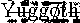
\includegraphics[scale=.75]{yuggoth_rlyeh.pdf}}}